\documentclass[a4paper,12pt]{article} % тип документа
\usepackage[margin=1in]{geometry} % Поля

%  Русский язык
\usepackage[warn]{mathtext}
\usepackage[T2A]{fontenc}			% кодировка
\usepackage[utf8]{inputenc}			% кодировка исходного текста
\usepackage[english,russian]{babel}	% локализация и переносы
% Математика
\usepackage{amsmath,amsfonts,amssymb,amsthm,mathtools} 
\usepackage{wasysym}
%%%
\usepackage{graphicx}

\usepackage{tabularx}

\usepackage{gensymb} % знак градуса
\usepackage{enumitem} % изменить список enumerate
\usepackage{placeins} % \FloatBarrier

\renewcommand{\thesection}{\Roman{section}} 
\renewcommand{\thesubsection}{\roman{subsection}}


\begin{document}

\newcolumntype{Y}{>{\centering\arraybackslash}X} %new tabularx


%титул

\begin{center}
{\LARGE Московский Физико-Технический Институт}
\\
{\large Физтех-школа электроники, фотоники и молекулярной физики }
\\
\vspace{8cm}
{\LARGE Отчёт по лабораторной работе:}
\\
{\Huge Масс спектроскопия остаточных газов. Квадрупольный масс-анализатор} 
\\
\vspace{5cm}
\raggedright 
\hspace{8cm}{\large Выполнили работу студенты }\\
\hspace{8cm}{\large группы Б04-005:}\\
\hspace{8cm}{\large Давыдов Владислав}\\
\hspace{8cm}{\large Карташов Констанин}\\
\hspace{8cm}{\large Корнеев Николай}\\

\vspace{\fill}
\center
{\large Долгопрудный 2022}

\end{center}

\newpage


\section{Анотация}

\paragraph{Цель работы:} 
Исследовать масс-спектр остаточных газов в вакуумной установке. Снять временную масс-спектрограмму для напускания и накачки газов. Расшифровать масс-спектрограммы.

\paragraph{Оборудование:}
\begin{itemize}
\renewcommand{\labelitemi}{$\triangleright$}
\itemsep0em
\item Установка VTS (Vacuum Training System) с квадрупольным масс-анализатором.
\item Персональный компьютер.
\end{itemize}




\medskip\hrule\medskip

\section{Масс-спектры остаточных газов}

\paragraph{} Мы провели 5 измерений с интервалом по времени в 6 минут, со следующими параметрами:

\begin{table}[h]
\centering
\begin{tabular}{|l|l|l|l|l|l|l|}
\hline
№ & $t_\text{окр}$, \degree С & $t_\text{турб}$, \degree С & $I_\text{турб}$, А & $W$, об/мин & $P \cdot 10^{-6}$, торр & $P_\text{qd} \cdot 10^{-9}$,  торр \\
\hline
1 & 28 & 41 & 0.23 & 42070 & 4.60 & 11 \\
\hline
2 & 29 & 41 & 0.23 & 42070 & 4.30 & 10 \\
\hline
3 & 29 & 42 & 0.22 & 42070 & 4.10 & 10 \\
\hline
4 & 29 & 43 & 0.23 & 42070 & 3.90 & 9.7 \\
\hline
5 & 30 & 43 & 0.22 & 42070 & 3.80 & 9.4 \\
\hline
\end{tabular}
\caption{Параметры при которых проведены измерения}
\label{tab1}
\end{table}

\paragraph{} Масс-спектры измерений из табл. \ref{tab1} в виде гистограммы на рис. \ref{spect1}-\ref{spect5}.

\begin{figure}[h]
\begin{center}
\begin{minipage}[h]{7cm}
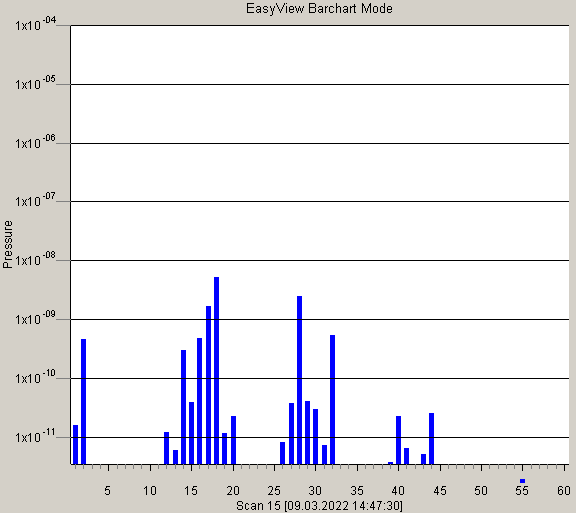
\includegraphics[width=7cm]{spect_1.png}
\caption{Измерение 1} 
\label{spect1}
\end{minipage}
\hfill
\begin{minipage}[h]{7cm}
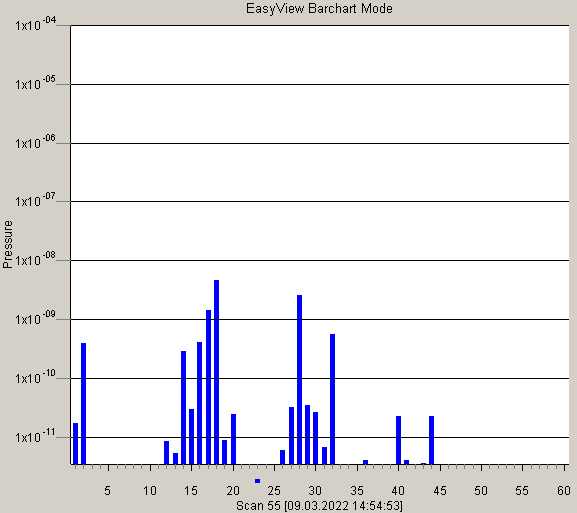
\includegraphics[width=7cm]{spect_2.png}
\caption{Измерение 2}
\label{spect2}
\end{minipage}
\end{center}
\end{figure}

\begin{figure}[h]
\begin{center}
\begin{minipage}[h]{7cm}
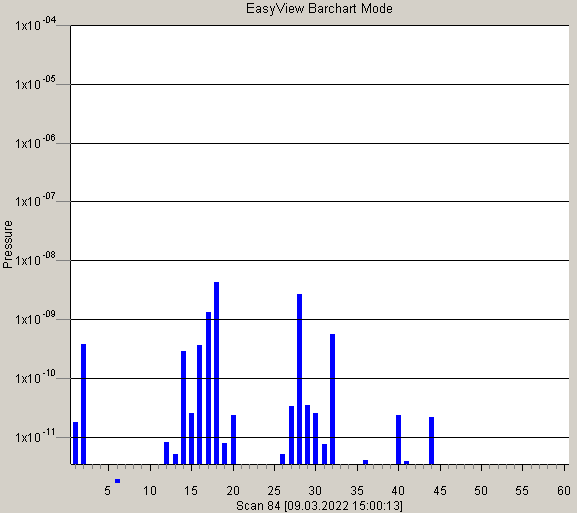
\includegraphics[width=7cm]{spect_3.png}
\caption{Измерение 3} 
\label{spect3}
\end{minipage}
\hfill
\begin{minipage}[h]{7cm}
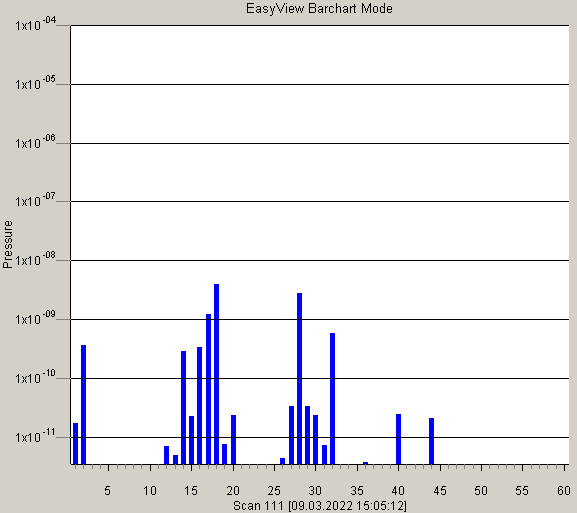
\includegraphics[width=7cm]{spect_4.png}
\caption{Измерение 4}
\label{spect4}
\end{minipage}
\end{center}
\end{figure}

\begin{figure}[h]
\center
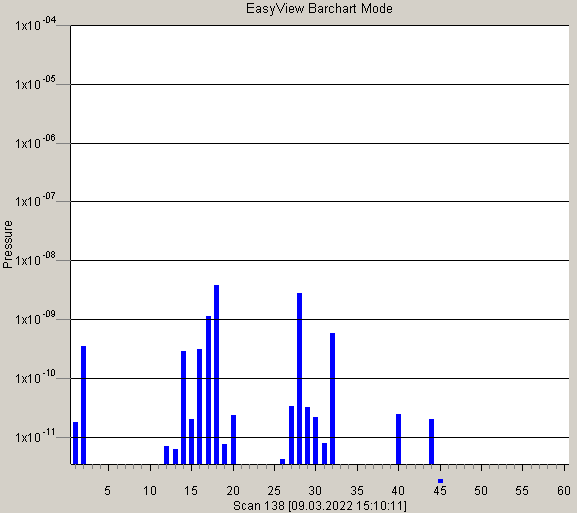
\includegraphics[width=7cm]{spect_5.png}
\caption{Измерение 5}
\label{spect5}
\end{figure}

\paragraph{} На масс-спектрах видно несколько пиков соответствующих массам:
\begin{itemize}
\renewcommand{\labelitemi}{$m_0 = $}
\itemsep0em
\item 2 -- водород (H$_2$)
\item 14 -- атомарный азот (N)
\item 16 -- атомарный кислород (O)
\item 17 -- аммиак (NH$_3$)
\item 18 -- вода (H$_2$O) -- самый большой пик
\item 28 -- молекулярный азот (N$_2$)
\item 32 -- молекулярных кислород (O$_2$)
\item 40 -- аргон (Ar)
\item 44 -- углекислый газ (CO$_2$)
\end{itemize}

\paragraph{Скорость откачки для различных газов.}
По графиками нескольких измерений видим, что парциальные давления для различных газов убывают с различной скоростью. Для более подробного изучения этих скоростей снимем временную масс-спектрограмму для нескольких пиков. 

Сначала проведём натекание, а затем проведём откачу. По временной масс-спектрограмме посмотрим с какими относительными скоростями меняются парциальные давления газов. Временная масс-спектрограмма показана на рис. \ref{time-spect}.

\begin{figure}[h]
\center
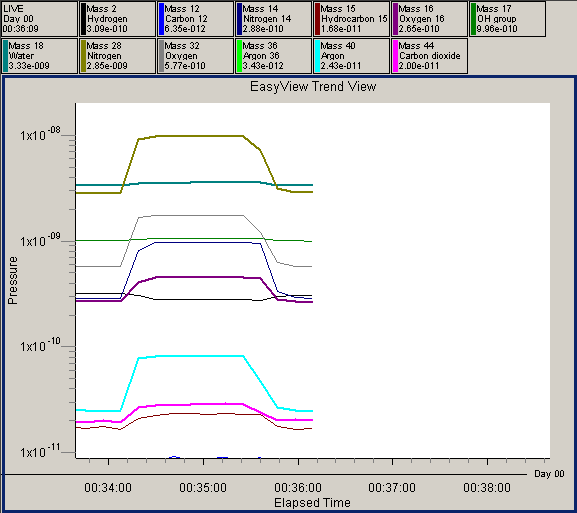
\includegraphics[width=10cm]{time-spect.png}
\caption{Временная масс-спектрограмма}
\label{time-spect}
\end{figure}

\paragraph{} По рис. \ref{time-spect} видим, что при напускании с одинаковой скоростью увеличивается парциальное давление газов с массами:
\begin{itemize}
\renewcommand{\labelitemi}{$m_0 = $}
\itemsep0em
\item 28, 32, 14, 40 -- быстрее всего,
\item 16, 44, 15 -- помедленнее,
\item 18, 17 -- почти не меняются,
\item 2 -- наоборот, уменьшается.
\end{itemize}

При откачке с одинаковой скоростью уменьшается давление газов с массами:

\begin{itemize}
\renewcommand{\labelitemi}{$m_0 = $}
\itemsep0em
\item 14 -- быстрее всего
\item 28, 32, 14, 40 -- немного помедленнее,
\item 16, 44, 15 -- помедленнее,
\item 18, 17 -- почти не меняются,
\item 2 -- наоборот, увеличивается.
\end{itemize}

Видим, что откачка и накачка происходит с для разов с одинаковыми относительными скоростями.

\medskip\hrule\medskip

\end{document}
